% !TeX root = main.tex
\documentclass[titlepage, 12pt]{article}
\usepackage{graphicx} % Required for inserting images
\usepackage{booktabs}
\usepackage[style=spanish]{csquotes}
\usepackage[T1]{fontenc}
\usepackage[main=spanish]{babel}
\usepackage{setspace}
\usepackage[a4paper, total={6in, 9.5in}]{geometry}
\usepackage[title]{appendix}
\usepackage[authordate, backend=biber]{biblatex-chicago}
\usepackage{xurl}
\usepackage{hyperref}
\usepackage{enumerate}
\usepackage{makecell}
\usepackage{subcaption}
\usepackage{float}
\usepackage{amsmath}
\usepackage[acronym,nonumberlist]{glossaries}
\makeglossaries

\newacronym{adf}{ADF}{\textit{Augmented Dickey-Fuller}}
\newacronym{bce}{BCE}{Banco Central Europeo}
\newacronym{boe}{BoE}{Banco de Inglaterra}
\newacronym{boj}{BoJ}{Banco de Japón}
\newacronym{cpi}{CPI}{\textit{Consumer Price Index}}
\newacronym{hicp}{HICP}{\textit{Harmonised Index of Consumer Prices}}
\newacronym{iofc}{IOFC}{\textit{Intermediate other financial corporation}}
\newacronym{kpss}{KPSS}{Kwiatkowski-Phillips-Schmidt-Shin}
\newacronym{mmt}{MMT}{\textit{Modern Monetary Theory}}
\newacronym{mpc}{MPC}{Comité de Política Monetaria}
\newacronym{nber}{NBER}{\textit{National Bureau of Economic Research}}
\newacronym{ofc}{OFC}{\textit{Other financial corporation}}
\newacronym{oiofc}{OIOFC}{\textit{Other intermediate other financial corporation}}
\newacronym{pib}{PIB}{Producto Interior Bruto}
\newacronym{qe}{QE}{\textit{Quantitative Easing}}
\newacronym{snb}{SNB}{\textit{Schweizerische Nationalbank}}
\newacronym{sebc}{SEBC}{Sistema Europeo de Bancos Centrales}
\newacronym{tfeu}{TFEU}{\textit{Treaty on the Functioning of the European Union}}
\newacronym{tecg}{TECG}{\textit{Tratado de Estabilidad, Coordinación y Gobernanza en la Unión Económica y Monetaria}}

\bibliography{bibliography.bib}
\title{Teoría cuantitativa del dinero en el mundo: oferta monetaria e inflación}
\author{Miguel González Calvo}
\date{Septiembre 2024}
\makeatletter

\begin{document}

\begin{titlepage}
    \centering
    {\bfseries\LARGE Universidad de las Hespérides \par}
    \vspace{1cm}
    {\scshape\Large Máster en Economía \par}
    \vspace{0.5cm}
    {\Large Curso 2023-2024 \par}
    \vspace{3cm}
    {\scshape\Huge \@title \par}
    \vspace{3cm}
    {\itshape\Large Trabajo Fin de Máster \par}
    \vfill
    {\Large Autor: \par}
    {\Large \@author \par}
    \vspace{2cm}
    {\Large Tutor: \par}
    {\Large Juan E. Castañeda \par}
    \vfill
    {\Large \@date \par}
\end{titlepage}
\makeatother

\spacing{1.5}
\pagenumbering{roman}

\tableofcontents
\newpage
\listoffigures
\listoftables

\newpage
\section*{Resumen}
Las diversas políticas monetarias adoptadas por los principales bancos centrales tuvieron efectos diferentes sobre la inflación durante la pandemia de COVID-19 y, especialmente, después de ella. Mientras que algunos países como Suiza y Japón registraron tasas de inflación anuales moderadas por debajo del 3,5\% (medidas por sus respectivos Índices de Precios al Consumo), no ocurrió lo mismo en otras zonas monetarias como Estados Unidos, la zona euro o el Reino Unido.

En los últimos años, en el mundo académico se han utilizado enfoques teóricos para explicar los orígenes de la inflación, entre ellos la teoría cuantitativa del dinero, el nuevo marco keynesiano, la teoría monetaria moderna y la teoría fiscal del nivel de precios. Dado que los principales bancos de las áreas monetarias y países mencionados aplicaron políticas con notables diferencias en términos de agregados monetarios amplios correlacionadas con resultados de inflación diversos, la teoría cuantitativa \enquote{amplia} del dinero puede ser un marco teórico adecuado para analizar el efecto de los agregados monetarios amplios sobre la inflación.

Por lo tanto, un análisis empírico como el que se presentará en este trabajo puede llevar a conclusiones relevantes sobre la posibilidad de utilizar las variaciones de los agregados monetarios y de la velocidad del dinero para establecer un vínculo con la inflación. Se utiliza un modelo de cambio de régimen (\textit{Markov-switching model}) para comprobar el impacto de las magnitudes monetarias (cambios en la oferta monetaria y en la velocidad del dinero) sobre la inflación para Suiza, Japón, Estados Unidos, la Eurozona y el Reino Unido.

El hecho de que se utilicen distintas zonas monetarias para el presente análisis permite un estudio multi-regional y multidivisa de las relaciones entre los agregados monetarios, la velocidad del dinero y la inflación.

Del análisis realizado para todas las áreas monetarias mencionadas se derivan principalmente dos conclusiones relevantes: primero, los cambios en la velocidad de circulación del dinero son estacionarios presentando un valor medio negativo y relativamente uniforme entre estas, con una variación similar; segundo, los cambios en la oferta monetaria en sentido amplio presentes y pasados son significativos a la hora de explicar cambios en el nivel de precios de las diferentes áreas monetarias.
\newpage
\begin{otherlanguage}{english}
  \section*{Abstract}
  Diverse monetary policies taken by leading central banks did have different effects on inflation during and especially after the COVID-19 pandemic. While certain countries such as Switzerland and Japan registered moderate annual inflation rates under 3.5\% (as measured by their respective Consumer Price Index), that was not the case for other monetary areas such as the United States, the Eurozone, or the United Kingdom.

  In the last years, theoretical approaches have been used in academia to explain the origins of inflation, including the quantity theory of money, the new Keynesian framework, the modern monetary theory, and the fiscal theory of the price level. Since the leading banks from the aforementioned monetary areas and countries implemented policies with remarkable differences in terms of broad money aggregates correlating with diverse inflation results, the \enquote{broad} quantitative theory of money can be a suitable theoretical framework to analyze the effect of broad monetary aggregates on inflation.

  Therefore, an empirical analysis such as the one to be presented in this publication can lead to relevant conclusions about the possibility of using changes in monetary aggregates and money velocity in order to establish a link to inflation. A regime-switching model (Markov-switching model) is used to test the impact of the monetary variables (changes in money quantity and money velocity) on inflation for Switzerland, Japan, the United States, the Eurozone, and the United Kingdom.

  The fact that different monetary areas are used for the present analysis allows for a multi-region, multi-currency study of relationships between monetary aggregates, money velocity, and inflation.

  From the analysis carried out for all the monetary areas mentioned above, two main conclusions are relevant: first, changes in the velocity of money circulation are stationary and have a negative and relatively uniform mean value among them, with a relatively similar variation among them; second, present and past changes in the broad money supply are significant in explaining changes in the price level of the different monetary areas.
\end{otherlanguage}

\newpage
\printglossary[type=acronym]

\newpage
\pagenumbering{arabic}

\section{Introducción}
Las elevadas tasas de inflación que han seguido a las diversas respuestas de diferentes bancos centrales a la crisis del COVID-19 plantean la cuestión acerca de si el marco teórico que manejan bancos centrales en diversas economías mundiales son acertados a la hora de predecir la inflación en función de la implementación concreta de la política monetaria por parte de los mismos.

Jerome Powell, el 23 de febrero de 2021, respondiendo al senador republicano de los Estados Unidos en el \enquote{Semiannual Monetary Policy Report to the Congress} ante el \textit{Committee on Banking, Housing, and Urban Affairs}:
\begin{displayquote}
    \begin{otherlanguage}{english}
        Well, when you and I studied economics a million years ago, M2 and monetary aggregates generally seemed to have a relationship to economic growth… that classic relationship between monetary aggregates and economic growth and the size of the economy, it just no longer holds… so something we have to unlearn, I guess. \autocite{powell2021a}.
    \end{otherlanguage}
\end{displayquote}
Además, el 1 de diciembre del mismo año añadía ante el \textit{House of Representatives’ Committee of Financial Services}:
\begin{displayquote}
    \begin{otherlanguage}{english}
        Now, we think more of just the imbalances between supply and demand in the real economy rather than monetary aggregates. … It’s been a different economy and a different financial system for some time,” \autocite{powell2021b}.
    \end{otherlanguage}
\end{displayquote}

Milton Friedman, por el contrario, ya planteaba décadas atrás la ya célebre tesis contraria:
\begin{displayquote}
    \begin{otherlanguage}{english}
        Inflation is always and everywhere a monetary phenomenon, in the sense that it is and can be produced only by a more rapid increase in the quantity of money than in output. \autocite[24]{friedman1970}.
    \end{otherlanguage}
\end{displayquote}

Se plantea la exploración, por tanto, de alternativas a dichos marcos teóricos con el fin de descubrir relaciones causales significativas entre los cambios en la velocidad de circulación del dinero y agregados monetarios, y la inflación registrada en diferentes áreas monetarias a nivel mundial.

\section{Materiales y métodos}

\subsection{Revisión bibliográfica}

A raíz de la implementación de una política monetaria expansiva en diferentes áreas monetarias, han sido varios los economistas que han alertado de una potencial inflación antes de que esta se registrara analizando el comportamiento de la oferta monetaria y de los cambios en la demanda de dinero durante y tras la crisis del COVID-19: \cite{castaneda2020}, \cite{congdon2020}.

Precisamente la influencia en los cambios en la oferta monetaria y los diferentes mecanismos de transmisión monetaria han sido el foco de estudio de una abundante cantidad de publicaciones, especialmente en los autores denominados monetaristas, comenzando por la ya clásica publicación de \cite{friedman1956}.

En los últimos años, sin embargo, y a raíz de la inflación resultante tras la política monetaria adoptada por los principales bancos centrales en relación con la crisis del COVID-19, se ha estudiado intensivamente la relación entre los cambios en la oferta monetaria y la inflación. Ejemplo de ello es el trabajo de \cite{borio2023}, donde se establece tal relación con una aproximación similar a la de este trabajo contemplando dos regímenes: un régimen de baja inflación y un régimen de alta inflación. Nótese, sin embargo, que la constatación de esta relación no implica causalidad: se observa que los países con un crecimiento de la oferta monetaria más fuerte registraron tasas de inflación más altas.

Por otro lado, \cite{greenwood2021} distingue entre dos tipos de explicaciones para la inflación: las explicaciones \textit{ad-hoc} y las explicaciones monetarias. Se pone en duda la capacidad de explicación de algunas de estas explicaciones \textit{ad-hoc} tales como el consenso neo-keynesiano tras haber fracasado en la correcta predicción de resultados de inflación, mientras que se resalta la importancia de los cambios en la oferta de dinero en sentido amplio en su relación con la inflación.

\cite{reynard2023}, por su parte, estudia la respuesta de los diferentes bancos centrales en términos de variación de sus respectivos balances y la inflación registrada. Se propone una relación entre inflación y oferta monetaria en sentido amplio usando como marco teórico la teoría cuantitativa del dinero. Se indica, asimismo, la importancia de la elección del agregado monetario a tratar, proponiendo el uso de agregados monetarios amplios.

Con relación a esta última cuestión, \cite{bordo2021} concluye que el multiplicador de la base monetaria no es estable comparando los agregados MB y M2 así como las consecuencias relativas a la inflación. Además, se hace un recorrido histórico de diferentes episodios de expansión fiscal y se analizan los resultados de las mismas en términos de cambio en el nivel de precios.

Es por ello por lo que se plantea la cuestión relativa a las limitaciones de las herramientas de las que disponen los bancos centrales para diseñar la política monetaria. A este respecto, \cite{congdon2021} analiza estas limitaciones para diseñar e implementar herramientas concretas de política monetaria sin conllevar inflación asociada.

Desde el punto de vista de metodología cuantitativa, una de las publicaciones que han explorado esta cuestión recientemente ha sido el de Castañeda y Cendejas, que \enquote{evalúa si los cambios en la velocidad de circulación del dinero y el crecimiento monetario (ampliamente) definido explica patrones de inflación a largo plazo en los Estados Unidos} \autocite[2]{castaneda2023}, concluyendo que, en efecto, ambas magnitudes sí tienen relevancia a la hora de explicar la inflación en el largo plazo.

La aplicación de metodologías cuantitativas para explicar la relación entre la oferta monetaria y la inflación ha sido profusa: a modo de ejemplo, \cite{amisano2013} usan un modelo markoviano con cambio de régimen similar al usado por Castañeda y Cendejas. Del mismo modo que se pretende en este trabajo, se expone la utilización del modelo para diferentes economías, siendo en ese caso la Eurozona, Alemania, los Estados Unidos, el Reino Unido y Canadá para un período de tiempo desde la década de 1960 hasta ese momento. Además, \cite{anderson2017} expone análisis similares a los de este trabajo correspondientes a la velocidad de circulación del dinero en términos de estacionariedad, y se usan modelos empíricos con el fin de modelar la demanda de dinero en sentido amplio en los Estados Unidos desde la Gran Depresión.

\subsection{La cuestión de los agregados monetarios}

Una de las cuestiones clave en torno al monetarismo es respectiva a la elección de un determinado agregado monetario. Nótese que, en general, pueden tomarse diferentes agregados que comprenden muy diversas magnitudes monetarias. A continuación, se listan algunas de ellas \autocite{oecd}:
\begin{itemize}
    \item \textbf{M0, MB o base monetaria:} reservas en el banco central y efectivo en circulación.
    \item \textbf{M1:} efectivo en circulación (billetes de banco y monedas) y depósitos a un día (\textit{overnight deposits}).
    \item  \textbf{M2:} suma de M1, los depósitos a plazo de hasta dos años y depósitos disponibles con preaviso de hasta tres meses (\textit{deposits redeemable at notice}).
    \item \textbf{M3 o dinero en sentido amplio:} suma de M2, cesiones temporales (\textit{repurchase agreements}), participaciones en fondos del mercado monetario (\textit{money market fund shares/units}) y títulos de deuda de hasta dos años (\textit{debt securities}).
\end{itemize}

Debido al hecho de que cada agregado monetario tiene un tamaño diferente y una relación diferentes con diversas variables macroeconómicas, el mecanismo de transmisión monetaria no puede ser el mismo. De hecho, que la causalidad entre el exceso o el defecto de dinero y las decisiones de gasto y de portafolio de activos se cumple para el dinero en sentido amplio, pero no para el dinero en sentido estrecho.  \autocite[137]{congdon2024}. Es por ello que en el presente trabajo se toman los agregados monetarios correspondientes al dinero en sentido amplio como medida de oferta monetaria.

\newpage
\begin{figure}
    \centering
    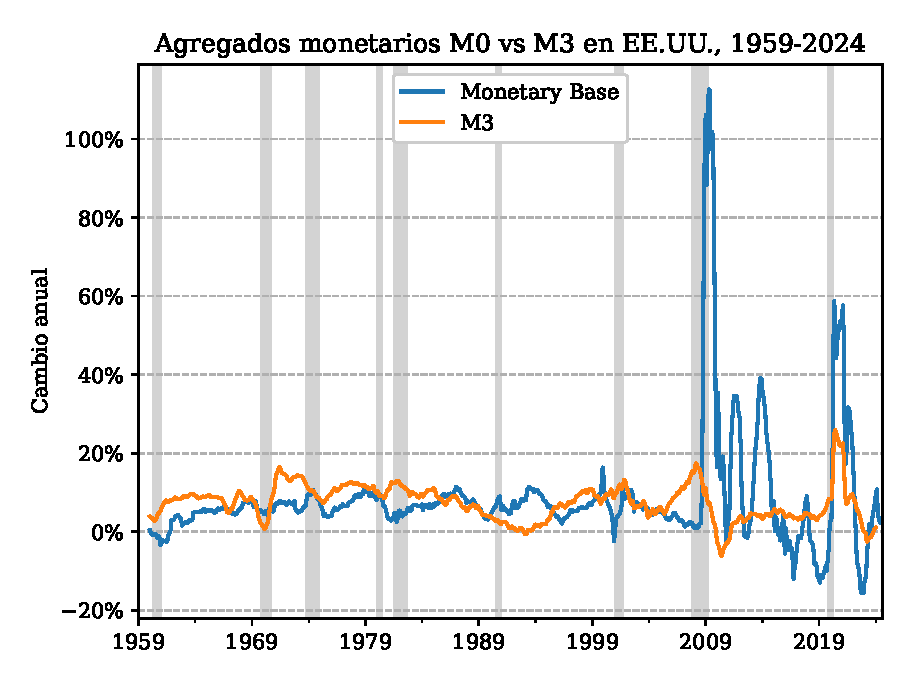
\includegraphics[width=.8\textwidth]{plots/broad-vs-narrow-money.eps}
    \caption{Agregado monetario estrecho (base monetaria, M0) vs. dinero en sentido amplio (M3) en los Estados Unidos. Elaboración propia.}
    \label{fig:broad-vs-narrow-money}
\end{figure}

Nótese, además, y tal como muestra \cite[76]{bordo2021}, que la relación entre el dinero en sentido amplio y el dinero en sentido estrecho no es ni constante ni sus variaciones coinciden en signo. Tal como muestra la Figura~\ref{fig:broad-vs-narrow-money}, durante la crisis financiera de 2008 se produjeron aumentos en la base monetaria mientras que el dinero en sentido amplio se reducía; en cambio, durante la crisis del COVID-19 ambas se comportaron con aumentos paralelos.

Es de especial interés el trato de los importes correspondientes a la compensación interbancaria. Los bancos almacenan reservas de dinero con el fin de destinarlas a potenciales compensaciones en el mercado interbancario. Ahora bien, estos pagos son de carácter puramente financiero; dado que no se realizan intercambios de bienes ni de servicios con estos importes, no tienen un efecto en la demanda agregada:

\begin{displayquote}
    \begin{otherlanguage}{english}
        Such reserves, which are fully convertible into legal tender, do constitute ‘money’ for the banking industry, but only for it. Interbank settlement is largely for the purpose of matching up accounts and is purely financial in character. No goods and services, and no payments for factors of production, are involved, and no effect on the expenditure-output flow or aggregate demand follow interbank settlement. \autocite[41]{congdon2024}
    \end{otherlanguage}
\end{displayquote}

De tal modo, M4 incluye el dinero en sentido amplio (\textit{broad money}), mientras que M4x se corresponde con el dinero en sentido amplio excluyendo las \acrfull{iofc} \autocite[41]{congdon2024}. Por ello en el caso del Reino Unido se usará M4x como agregado monetario para el análisis expuesto.

\subsection{Teorías alternativas}

La inflación ha sido un fenómeno harto estudiado en el campo de la economía política. No obstante, no existe un consenso sobre qué variables impactan en la misma; es por ello que a lo largo de los siglos han ido surgiendo corrientes económicas que la han atribuido a diferentes factores. Así como el monetarismo otorga un papel esencial a la hora de explicar la inflación a la oferta de dinero, no es así en otra serie de teorías alternativas que en este trabajo se pretenden esbozar.

\subsubsection{Modelo Neokeynesiano}\label{modelo-neokeynesiano}
La determinación de la política monetaria a implementar por parte de los bancos centrales de diferentes economías ha sido fruto de numerosos debates a lo largo de los últimos años. A partir de esta cuestión han surgido reglas monetarias tales como la Regla de Taylor, y diferentes perspectivas en función de qué hipótesis se toman como punto de partida. Algunas de estas hipótesis tienen una cierta relación con el pensamiento de John Maynard Keynes, y precisamente por la incorporación de elementos tales como la rigidez de precios nominales u otro tipo de rigideces (a modo de ejemplo en la demanda de dinero), se denomina tales enfoques como una \enquote{perspectiva neokeynesiana} \autocite[1662]{clarida1999}.

Uno de los modelos más destacables en la \enquote{perspectiva neokeynesiana} es el presentado precisamente por Richard Clarida, Jordi Galí y Mark Gertler (1999). En este, se relaciona la inflación con dos factores determinantes, a saber: las expectativas de inflación y el \enquote{\textit{output gap}} o brecha de producción (la diferencia entre la producción potencial y la producción real). De este modo, no se establece, al igual que en el modelo planteado en este trabajo, una relación directa entre la implementación de política monetaria en forma de variación de la oferta de dinero y la inflación registrada, sino que esta se atribuye a otros factores determinantes.

\subsubsection{Teoría fiscal del nivel de precios}
Una de las cuestiones esenciales de la teoría monetaria es explicar la razón por la cual existe confianza en el dinero fiat por contraposición al dinero con convertibilidad en activos reales, y una de las explicaciones más aceptadas en la comunidad académica es la chartalista: por la capacidad del dinero fiat de extinguir deudas con el Estado. Tal como expone \cite{ben_gad2023}, es este principio el que da lugar a dos corrientes que convergen en este punto y divergen en las explicaciones particulares, a saber: la teoría monetaria moderna y la teoría fiscal del nivel de precios.

Uno de los máximos exponentes de la teoría fiscal del nivel de precios es John H. Cochrane, que expone en el libro homónimo \textit{The Fiscal Theory of the Price Level} \autocite*{cochrane2023} los principios de la misma, que pueden resumirse en que el valor de la moneda fiat depende fundamentalmente de los flujos de caja esperados por parte del Estado, esto es, del conjunto de déficits o superávits esperados futuros del mismo. De este modo, la inflación no es considerada un fenómeno puramente monetario, sino que depende del pasivo estatal: \enquote{inflation is not a monetary phenomenon but rather a government liability phenomenon} \autocite[305]{ben_gad2023}.

\subsubsection{Teoría monetaria moderna}
La \acrfull{mmt} es una teoría alternativa al monetarismo correspondiente al reconocimiento del Estado como monopolio de emisión de dinero, y sus ideas pueden resumirse en dos tesis principales \autocite{rallo2015}: primero, que en presencia de recursos ociosos el Estado tiene la posibilidad de usar la oferta de moneda sin producirse efectos perniciosos para la economía o inflación; y segundo, que el dinero es una criatura del Estado. Es necesaria, por ello, la constatación del íntimo vínculo entre la teoría monetaria moderna y el chartalismo, y, más en concreto, el neochartalismo (recuérdese la célebre afirmación de Georg Friedrich Knapp \enquote{el dinero es una criatura de la ley}).

En concreto, el autoproclamado fundador de la teoría monetaria moderna, Warren Mosler, en Los siete fraudes inocentes capitales de la política económica (2010) expone siete fraudes de la política económica y la contraparte explicación usando la teoría correspondiente, basados en el principio fundamental de monopolio público:

\begin{displayquote}
    \acrshort{mmt} alone recognizes that the US Government and its agents, including its regulated commercial banks, are the sole supplier of that which it demands for payment of taxes \autocite{mosler2020}
\end{displayquote}

Y siguiendo la teoría propuesta, se alcanza uno de los corolarios más importantes: el emisor de una moneda no puede enfrentarse a limitaciones de carácter financiero. Tal como exponen William Mitchell, Randall Wray, L y Martin Watts (2019): \enquote{put simply, a country that issues its own currency can never run out and can never become insolvent in its own currency}.

Dejando a un lado las consecuencias para el desempleo y otros aspectos económicos, es de interés para este trabajo exponer sucintamente las consecuencias derivadas para la inflación: según la teoría monetaria moderna de acuerdo con las exposiciones de \cite{mitchell2019} y \cite{kelton2020}, la financiación de tipo monetaria del gasto público no ha de causar inflación, siempre y cuando la economía tenga recursos ociosos donde destinar este gasto.

No obstante, la evidencia empírica no sustenta esta tesis, sino que la monetización de deuda a través de un incremento excesivo de la oferta monetaria con respecto al nivel específico de demanda de dinero resulta empíricamente en inflación. Es destacable, en este aspecto, el trabajo de \cite{castaneda2021}, explicando por qué la teoría monetaria moderna no puede proveer crecimiento económico sostenido y baja inflación.


\subsection{Análisis cuantitativo}
El presente trabajo pretende evaluar si los cambios en la velocidad de circulación del dinero y en la cantidad de dinero (en forma de agregados monetarios concretos) tienen impacto en la inflación a largo plazo usando datos de diferentes áreas monetarias.

De este modo se presenta un estudio controlado en diferentes economías a nivel mundial de la influencia de los cambios en la velocidad de circulación de dinero y los agregados monetarios amplios (\enquote{broad money}) en el \acrfull{cpi}.

Para conseguir este fin se usará la metodología cuantitativa presentada en \autocite{castaneda2023}, extendiendo el análisis desde únicamente los Estados Unidos hasta otras economías que han presentado un diferente comportamiento en términos de implementación de política monetaria y de inflación registrada: la Eurozona, el Reino Unido, Suiza y Japón.

El período de tiempo de análisis se escoge de acuerdo con el máximo alcanzable con la disponibilidad de los datos correspondientes a las tres magnitudes de análisis (agregados monetarios amplios, PIB nominal y tasa de inflación) para las cinco áreas monetarias de interés.

\subsubsection{Variables y datos utilizados}
Se disponen de las magnitudes correspondientes a los diferentes agregados monetarios, así como al producto interior bruto nominal. Así, usando la ecuación de intercambio es posible calcular la velocidad de circulación del dinero para la moneda correspondiente:
\begin{equation}
    M_t\cdot v_t=P_t\cdot Y_t
\end{equation}
\begin{equation}
    v_t=\frac{P_t\cdot\ Y_t}{M_t}\
\end{equation}
Donde:
\begin{itemize}
    \item $M_t$ es la cantidad de dinero en circulación, correspondiente al agregado monetario que se vaya a tomar (en el caso de este trabajo se corresponde con las magnitudes M3 para los análisis de Estados Unidos, la Eurozona, Suiza y Japón y M4x para el Reino Unido).
    \item $v_t$ es la velocidad de circulación del dinero en el área monetaria correspondiente.
    \item $P_t$ es el nivel de precios en el área monetaria correspondiente.
    \item $Y_t$ es la producción real de la economía del área monetaria correspondiente.
\end{itemize}

De tal modo, se deriva que $P_t\cdot Y_t$ se corresponde con el producto interior bruto nominal del área monetaria correspondiente, siendo $Y_t$ el PIB real de la misma.

Para el análisis se tomarán las variaciones anuales logarítmicas en las magnitudes propuestas, de tal modo que se cumple:

\begin{equation}
    \Delta\log{v_t}=\Delta\log{\left(P_tY_t\right)}-\Delta\log{M_t}
\end{equation}

Los datos concretos utilizados para el estudio empírico y sus correspondientes fuentes pueden ser consultados al final de este trabajo en el Anexo~\ref{fuentes-de-informacion}.

\subsubsection{Análisis de estacionariedad}

Una de las conclusiones observadas por el análisis de \cite{castaneda2023} es el comportamiento estacionario de los cambios en la velocidad de circulación del dinero para el período observado en los Estados Unidos: aunque hay cambios significativos en la misma, se caracteriza por producirse recurrentemente una regresión a la media, explicándose porque “los valores de $\Delta\log{\left(P_tY_t\right)}$ y $\Delta\log{M_t}$ no siguen trayectorias divergentes por períodos de tiempo excesivamente largos” \autocite[8]{castaneda2023}. Así, la media a la que se regresa puede interpretarse como una situación de equilibrio económico y situaciones de desequilibrio (entre el crecimiento del PIB nominal y el crecimiento de la cantidad de dinero) cuando los cambios en la velocidad de circulación del dinero se alejan de la misma.

Una de las críticas más repetidas a lo largo de los últimos años al monetarismo corresponde a cambios significativos en la demanda de dinero, especialmente en las últimas décadas. Es por ello que se decide realizar un estudio de estacionariedad respecto a los cambios en la velocidad de circulación del dinero no sólo en los Estados Unidos, sino en las otras áreas monetarias de interés. Nótese, además, que la velocidad de circulación del dinero es inversamente proporcional a la demanda de dinero y puede tomarse como variable \enquote{proxy} para determinar su variación.

Se observa, asimismo, que los cambios en la velocidad de circulación del dinero no exhiben una media nula, sino que se distribuyen en torno a un valor medio $\mu_v$. Es por esto que se realizará un contraste de hipótesis para verificar que ese valor medio en efecto no es nula, planteándose:

$H_0$ (hipótesis nula): el valor medio de $\Delta\log{v_t}$ es $\mu_0=0$, $E\left[\Delta\log{v_t}\right]=\mu_v=0$.
\begin{equation}
    t_{\mathrm{score}}=\frac{\overline{\Delta\log{v_t}}-\mu_0}{s_{m\overline{\Delta\log{v_t}}}}
\end{equation}
%
Siendo:
\[s_{m\overline{\Delta\log{v_t}}}=\frac{s_{m\Delta\log{v_t}}}{\sqrt T}\]
%
y calculando el valor p por medio de la función de distribución:
\[\mathrm{valor-p}\left(x,\nu\right)=2\left(1-\mathrm{cdf}\left(x,\nu\right)\right)=1-2x\Gamma\left(\frac{\nu+1}{2}\right)\]
%
Donde $\nu=T-1$ y $x=t_{score}$.

Tras plantear y evaluar la hipótesis nula, se realizará un análisis de estacionariedad evaluando la existencia o no de raíces unitarias en la serie temporal. Para ello se recurrirá a la prueba de Dickey Fuller (Augmented Dickey-Fuller test), donde la hipótesis nula es que existe una raíz unitaria en la serie \autocite{dickey1979}.

\subsubsection{Modelo de regresión de Markov}
Con carácter general, un modelo de regresión de Markov con dos regímenes puede ser expresado como sigue:

\begin{align}
    \begin{split}
        y_t           & =\alpha_0+\alpha_1t+\sum\beta_ix_{i,t}+\sum\beta_{j,S_1}S_tx_{j,t}+\sum{\beta_{j,S_2}\left(1-S_t\right)x_{j,t}}+\varepsilon_t \\
        \varepsilon_t & \sim N\left(0,\sigma_{S_t}^2\right)
    \end{split}
\end{align}

Nótese que un modelo de regresión de Markov generalizado no tiene por qué tener dos estados, sino que se pueden disponer de $K$ estados diferentes. Dado que los modelos que se implementan disponen de dos estados ($K=2$), se cumple:

\begin{equation}
    S_{2,t}=\left(1-S_{1,t}\right)
\end{equation}

Y por simplicidad de notación se define el primer régimen como $S_t=S_{1,t}$ y el segundo como $S_{2,t}=1-S_t$.

De este modo se encuentran variables exógenas que son modeladas cambiando de régimen ($x_{i,t}$), así como variables exógenas que no son modeladas cambiando de régimen ($x_{j,t}$).

El modelado de tendencia puede ser realizado a través de una constante ($\alpha_0$), o a través de un modelo lineal con constante y/o pendiente ($\alpha_0+\alpha_1t$). Del mismo modo, la tendencia puede ser modelada con o sin cambio de régimen:

\begin{equation}
    y_t=\alpha_0+\alpha_1t+\varepsilon_t
\end{equation}

\begin{equation}
    y_t=\left(\alpha_{0,S_1}+\alpha_{1,S_1}t\right)S_t+\left(\alpha_{0,S_2}+\alpha_{1,S_2}t\right)\left(1-S_t\right)+\varepsilon_t
\end{equation}

Y si el proceso es homocedástico, la varianza será constante en el tiempo:
\begin{equation}
    \varepsilon_t\sim N\left(0,\sigma^2\right)
\end{equation}

\subsubsection{Velocidad de circulación del dinero}
En concreto, el modelo aplicado a la velocidad de circulación del dinero se expresa del siguiente modo:
%
\begin{align}
    \begin{split}
        \Delta\log{v_t} & =\beta_{\mathrm{recession}}d_{\mathrm{recession,t}}+\alpha_{S_1}S_t+\alpha_{S_2}\left(1-S_t\right)+\varepsilon_t \\
        \varepsilon_t   & \sim N\left(0,\sigma^2\right)
    \end{split}
    \label{eq:markov-v}
\end{align}
%
Donde:
\begin{itemize}
    \item $v_t$ es la velocidad de circulación del dinero.
    \item $d_{\mathrm{recession,t}}$ es una variable dicotómica que toma el valor 0 en períodos de expansión económica y 1 en períodos de recesión económica. Nótese, por tanto, $d_{\mathrm{recession,t}}\in\{0,1\}$.
    \item $S_t$ representa la predicción del régimen en el cual se encuentra la serie temporal en el instante temporal $t$. Nótese que en este modelo existen dos regímenes definidos, por lo que $S_t\in\{0,1\}$.
    \item $\beta_i$ son los coeficientes que serán determinados por el modelo.
    \item $\alpha_{S_k}$ son los coeficientes de tendencia por régimen.
    \item $\varepsilon_t$ es el residuo correspondiente al instante temporal t. Con las hipótesis planteadas, se deriva que los residuales están normalmente distribuidos con media nula y varianza constante: $\varepsilon_t\sim N\left(0,\sigma^2\right)$.
    \item $p_{ij}$ es la probabilidad de realizar una transición desde el régimen $i$ al régimen $j$.
\end{itemize}


\begin{equation}
    P\left(S_t=s_t\middle| S_{t-1}=s_{t-1}\right)=
    \begin{bmatrix}
        p_{00}   & p_{10}   \\
        1-p_{00} & 1-p_{10} \\
    \end{bmatrix}
\end{equation}


Nótese que se supone un proceso homocedástico donde la varianza se mantiene constante a lo largo del tiempo. Se propone como trabajo futuro realizar un análisis más exhaustivo de la evolución de la varianza en el tiempo para las diferentes áreas monetarias analizadas, así como en el caso de determinarse heterocedasticidad, implementarla en el modelo de regresión de Markov propuesto, de tal modo que los residuales no cobrarían la forma anteriormente propuesta sino $\varepsilon_t\sim N\left(0,\sigma_{S_t}^2\right)$. En la implementación del modelo correspondiente equivaldría a \texttt{switching\_variance=True} \autocite{statsmodels2024c}.

Los datos correspondientes a los períodos de expansión y recesión económica se corresponden con los picos y valles definidos por el National Bureau of Economic Research \autocite{nber2023}.


\begin{table}
    \centering
    \begin{tabular}{ll}
        \toprule
        Pico   & Valle  \\
        \midrule
        1857Q2 & 1858Q4 \\
        1860Q3 & 1861Q3 \\
        1865Q1 & 1867Q1 \\
        1869Q2 & 1870Q4 \\
        1873Q3 & 1879Q1 \\
        1882Q1 & 1885Q2 \\
        1887Q2 & 1888Q1 \\
        1890Q3 & 1891Q2 \\
        1893Q1 & 1894Q2 \\
        1895Q4 & 1897Q2 \\
        1899Q3 & 1900Q4 \\
        1902Q4 & 1904Q3 \\
        1907Q2 & 1908Q2 \\
        1910Q1 & 1911Q4 \\
        1913Q1 & 1914Q4 \\
        1918Q3 & 1919Q1 \\
        1920Q1 & 1921Q3 \\
        \bottomrule
    \end{tabular}
    \begin{tabular}{ll}
        \toprule
        Pico   & Valle  \\
        \midrule
        1923Q2 & 1924Q3 \\
        1926Q3 & 1927Q4 \\
        1929Q3 & 1933Q1 \\
        1937Q2 & 1938Q2 \\
        1945Q1 & 1945Q4 \\
        1948Q4 & 1949Q4 \\
        1953Q2 & 1954Q2 \\
        1957Q3 & 1958Q2 \\
        1960Q2 & 1961Q1 \\
        1969Q4 & 1970Q4 \\
        1973Q4 & 1975Q1 \\
        1980Q1 & 1980Q3 \\
        1981Q3 & 1982Q4 \\
        1990Q3 & 1991Q1 \\
        2001Q1 & 2001Q4 \\
        2007Q4 & 2009Q2 \\
        2019Q4 & 2020Q2 \\
        \bottomrule
    \end{tabular}
    \caption{Períodos de expansión y recesión económica de acuerdo con el National Bureau of Economic Reserach \autocite{nber2023}.}
\end{table}

\subsubsection{Inflación}
Se toman como variables exógenas las variables de interés, así como los retrasos de las mismas. Con el fin de simplificar la notación se usará el operador \enquote{lag} ($L$) de este modo:

\begin{equation}
    L^mx_t=x_{t-m}
\end{equation}

Asimismo, se usará una expresión polinómica para representar un conjunto de retrasos como sigue independiente de los cambios de régimen:

\begin{equation}
    \gamma\left(L\right)=\gamma_0+\gamma_1L+\gamma_2L^2+\cdots
\end{equation}
%
Y otras dos expresiones polinómicas (correspondientes a los $k\in\{1,2\}$ regímenes) para expresar los coeficientes a estimar por el modelo:
%
\begin{equation}
    \alpha_{S_k}\left(L\right)=\alpha_{0,S_k}+\alpha_{1,S_k}L+\alpha_{2,S_k}L^2+\cdots
\end{equation}
\begin{equation}
    \Delta\log{P_t}=\left[c_{S_1}+\alpha_{S_1}\left(L\right)\Delta\log{M_t}\right]S_t+\left[c_{S_2}+\alpha_{S_2}\left(L\right)\Delta\log{M_t}\right]\left(1-S_t\right)+\gamma\left(L\right)\Delta\log{v_t}+\varepsilon_t
    \label{eq:markov-cpi}
\end{equation}

\newpage
\section{Discusión y conclusiones}

\subsection{Marco institucional}
Desde las instituciones de las diferentes áreas monetarias se establecen marcos regulatorios que persiguen el mandato de la estabilidad de precios, así como marcar límites al endeudamiento público.

\subsubsection{Estados Unidos}
La estabilidad de precios se recoge como objetivo a perseguir en el \enquote{mandato plural} de la Reserva Federal, autoridad monetaria en los Estados Unidos.

Este mandato está regulado por las enmiendas del 16 de noviembre de 1977 (12 USC § 225a) a la Ley de la Reserva Federal de 1913. En este caso se trata de una ley del Congreso de los Estados Unidos que establece como objetivos de la Reserva Federal \enquote{el máximo empleo, precios estables, y tipos de interés de largo plazo moderados}. Por ello la Reserva Federal, para conseguir garantizar un nivel estable de precios, se esfuerza por mantener la inflación baja y estable, normalmente apuntando a una tasa de inflación anual de alrededor del dos por ciento.

En cuanto a los límites de déficit y deuda, el Congreso de Estados Unidos establece límites al endeudamiento del gobierno federal mediante legislación. El límite más conocido es el techo de deuda, que es la cantidad máxima de dinero que el gobierno está autorizado a pedir prestado para cumplir con sus obligaciones legales existentes, como el pago de facturas y el servicio de la deuda existente.

Cuando el gobierno alcanza el techo de deuda, el Congreso debe votar para aumentarlo y permitir que el gobierno siga endeudándose. No aumentar el techo de la deuda puede llevar al cierre del gobierno o al incumplimiento de sus obligaciones, lo cual puede tener graves consecuencias económicas.

Además, existen restricciones y directrices informales para el gasto deficitario, pero no se trata de límites estrictos como el techo de deuda. El nivel de gasto deficitario está influenciado por varios factores, incluidas las condiciones económicas, las consideraciones políticas y las decisiones de política fiscal tomadas por el Congreso y el presidente.

\subsubsection{Eurozona}

La legislación europea en términos de estabilidad de precios es compleja y está recogida en diferentes tratados firmados por los Estados miembros \autocite{lemos2023} y establece tanto un mandato general como condiciones específicas para los diferentes bancos centrales y para los gobiernos nacionales.

La estabilidad de precios se establece como mandato en el Tratado de Maastricht y posteriormente se consolidó en el Artículo 127 (1) del Tratado de Funcionamiento de la Unión Europea (parte tercera, título VIII, capítulo 2): \enquote{El objetivo principal del \acrfull{sebc}, denominado en lo sucesivo \enquote{SEBC}, será mantener la estabilidad de precios. Sin perjuicio de este objetivo, el \acrshort{sebc} apoyará las políticas económicas generales de la Unión con el fin de contribuir a la realización de los objetivos de la Unión establecidos en el artículo 3 del Tratado de la Unión Europea.}.

La estabilidad de precios también se recoge en el Artículo 140 del \acrfull{tfeu}: \enquote{el logro de un alto grado de estabilidad de precios, que deberá quedar de manifiesto a través de una tasa de inflación que esté próxima a la de, como máximo, los tres Estados miembros más eficaces en cuanto a la estabilidad de precios}. Además, indirectamente en el mismo artículo a través de los tipos de cambio requiriendo \enquote{el respeto, durante dos años como mínimo, sin que se haya producido devaluación frente al euro, de los márgenes normales de fluctuación que establece el mecanismo de tipos de cambio del sistema monetario europeo}, así como \enquote{el carácter duradero de la convergencia conseguida por el Estado miembro acogido a una excepción y de su participación en el mecanismo de tipos de cambio deberá verse reflejado en los niveles de tipos de interés a largo plazo}.

Sin embargo, no sólo se fijan condiciones relativas al banco central y a la emisión monetaria, sino también condiciones relativas al gobierno a través de la limitación del déficit público en el mismo artículo 140 del \acrshort{tfeu}: \enquote{las finanzas públicas deberán encontrarse en una situación sostenible, lo que quedará demostrado en caso de haberse conseguido una situación del presupuesto sin un déficit público excesivo, definido de conformidad con lo dispuesto en el apartado 6 del artículo 126}.

Posteriormente, a principios de 2013 entra en vigor el \acrfull{tecg} que, en su Pacto Presupuestario firmado por todos los Estados miembros excepto el Reino Unido y la República Checa, establece un límite mínimo estructural del 0,5 \% del \acrshort{pib}, con la salvedad de Estados con una deuda pública inferior al 60 \% del \acrshort{pib}, cuyo límite inferior sería del 1 \% del \acrshort{pib}.

En cuanto a la estrategia de la política monetaria del \acrfull{bce}, esta viene dada por la \enquote{Declaración sobre la estrategia de política monetaria del \acrshort{bce}}, publicada el 8 de julio de 2021 y sustituyendo a la anteriormente publicada en el año 2003. Así, se establece el HCIP como indicador a evaluar:

\begin{displayquote}
    El Consejo de Gobierno confirma que el Índice Armonizado de Precios de Consumo (IAPC) continúa siendo el indicador de precios adecuado para evaluar la consecución del objetivo de estabilidad de precios. \autocite{ecb2021}.
\end{displayquote}

Y se establece un límite a la inflación:
\begin{displayquote}
    El \acrshort{bce} se ha comprometido a fijar su política monetaria para asegurar que la inflación se estabilice en su objetivo del 2 \% a medio plazo. \autocite{ecb2021}.
\end{displayquote}

\subsubsection{Reino Unido}

En el Reino Unido el \acrfull{boe} fija la política monetaria para \enquote{mantener la inflación en el Reino Unido baja y estable} \autocite{boe}. Para ello, el \acrlong{boe} hace uso de dos herramientas para implementar la política monetaria: por un lado se usa el \textit{bank rate}, que es el tipo de interés que el Banco paga en depósitos diarios por entidades admitidas tales como bancos comerciales; por otro se contempla la compra de activos financieros tales como bonos a través de la expansión cuantitativa, \acrfull{qe}.

De acuerdo con el Banco, la inflación es \enquote{el objetivo primario de la política monetaria}, de tal modo que se persigue el objetivo que se le entrega al \acrshort{boe} desde el gobierno del Reino Unido (en la actualidad el objetivo está fijado en un dos por ciento).

La decisión correspondiente a la política monetaria a implementarse corresponde, por tanto, a nueve individuos que pertenecen al \acrfull{mpc}, que anuncian la política a adoptar ocho veces al año.

Para una visión crítica correspondiente a la política monetaria adoptada por parte del Banco de Inglaterra puede consultarse el capítulo noveno de \textit{The Quantity Theory of Money: A New Restatement} \autocite[109-129]{congdon2024}.

Es de interés señalar una de las principales diferencias entre la arquitectura institucional del Banco de Inglaterra y la de la Reserva Federal o del Banco Central Europeo: mientras que estas dos últimas instituciones son responsables de fijar sus propios objetivos de inflación, el Banco de Inglaterra no es autónomo en estos términos, sino que el objetivo de inflación es comunicado por el gobierno al propio banco.

\subsubsection{Suiza}

El \acrfull{snb} recibe el mandato de asegurar la estabilidad de precios tomando en consideración la evolución económica. A fin de alcanzar este objetivo, la estrategia de política moentaria del \acrshort{snb} se compone de tres elementos, a saber: la definición de estabilidad de precios, la previsión de inflación a medio plazo, y la definición del tipo de interés oficial del SNB \autocite{snb2024a}.

La descripción de los instrumentos de política monetaria de los que dispone el \acrshort{snb} están descritos en las \enquote{Guidelines of the Swiss National Bank on monetary policy instrument} \autocite{snb2024b}.

\subsubsection{Japón}
El \acrfull{boj} toma las decisiones correspondientes a la política monetaria y se encarga de implementarla con el fin de mantener la estabilidad de precios \autocite{boj2024a}.

El marco institucional establece a través del \enquote{Bank of Japan Act} que la política monetaria debe estar \enquote{encaminada a lograr la estabilidad de precios, contribuyendo así al sano desarrollo de la economía nacional}. En concreto, el Banco de Japón fija como objetivo un \enquote{objetivo de estabilidad de precios} establecido en 2013 por el mismo en un dos por ciento de cambio anual en el índice de precios al consumidor (CPI).

La política monetaria se define por parte de la \textit{Policy Board} en los \textit{Monetary Policy Meetings}, mientras que la implementación de la política monetaria se realiza a través de diferentes instrumentos operacionales tales como las operaciones del mercado monetario.

\subsection{Resultados cuantitativos}
La implementación de los modelos propuestos se ha realizado en Python usando los modelos implementados en la librería de statsmodels \autocite{statsmodels2024a}. La implementación concreta junto con el código producido puede ser consultado en el correspondiente repositorio online creado ex profeso \autocite{github2024}.

Una vista general de los cambios en la oferta de dinero en sentido amplio (M3 y M4x), así como de la tasa de inflación para las diferentes áreas monetarias puede ser consultada en la Figura~\ref{fig:m3-inflation}. Puede observarse cómo tras la fuerte subida repentina de la oferta de dinero en los Estados Unidos, en la Eurozona y en el Reino Unido le sigue un significativo incremento de la inflación, no constatándose un incremento de similar magnitud en el caso de Suiza o Japón.

La Figura~\ref{fig:magnitudes} muestra las diferentes magnitudes usadas para el análisis y los períodos de estudio para las áreas monetarias correspondientes: los Estados Unidos, la Eurozona, Suiza, el Reino Unido o Japón.

\begin{figure}
    \centering
    \begin{subfigure}[b]{0.49\textwidth}
        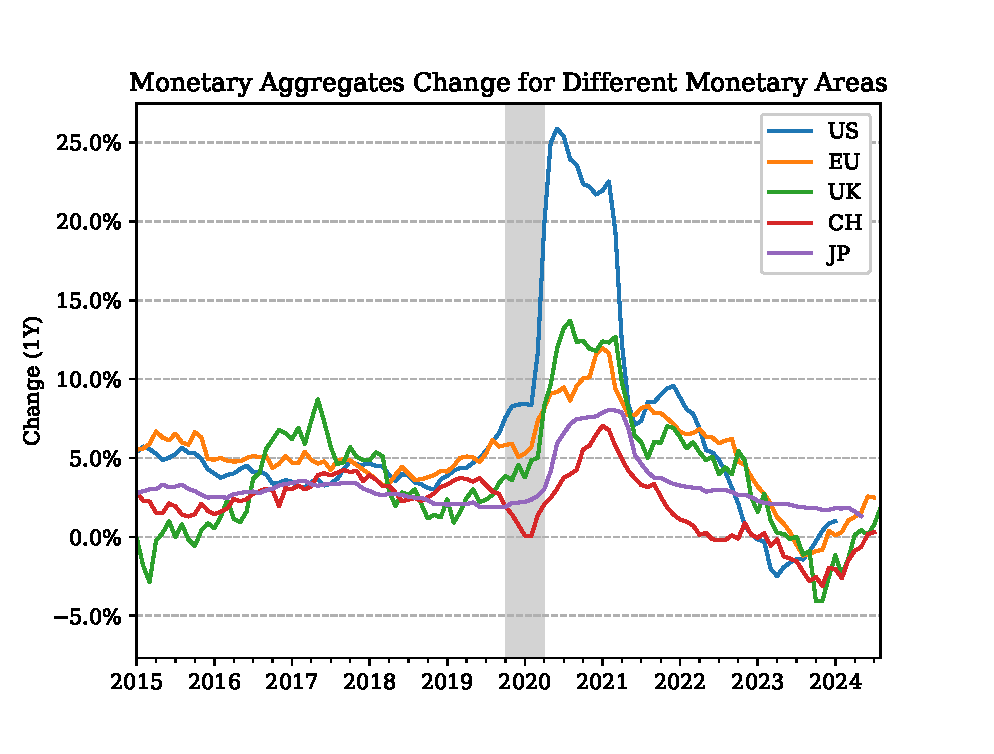
\includegraphics[width=\textwidth]{plots/money-supply.eps}
        \caption{Cambio anual en la cantidad de dinero en sentido amplio (M3 y M4x).}
    \end{subfigure}
    ~
    \begin{subfigure}[b]{0.49\textwidth}
        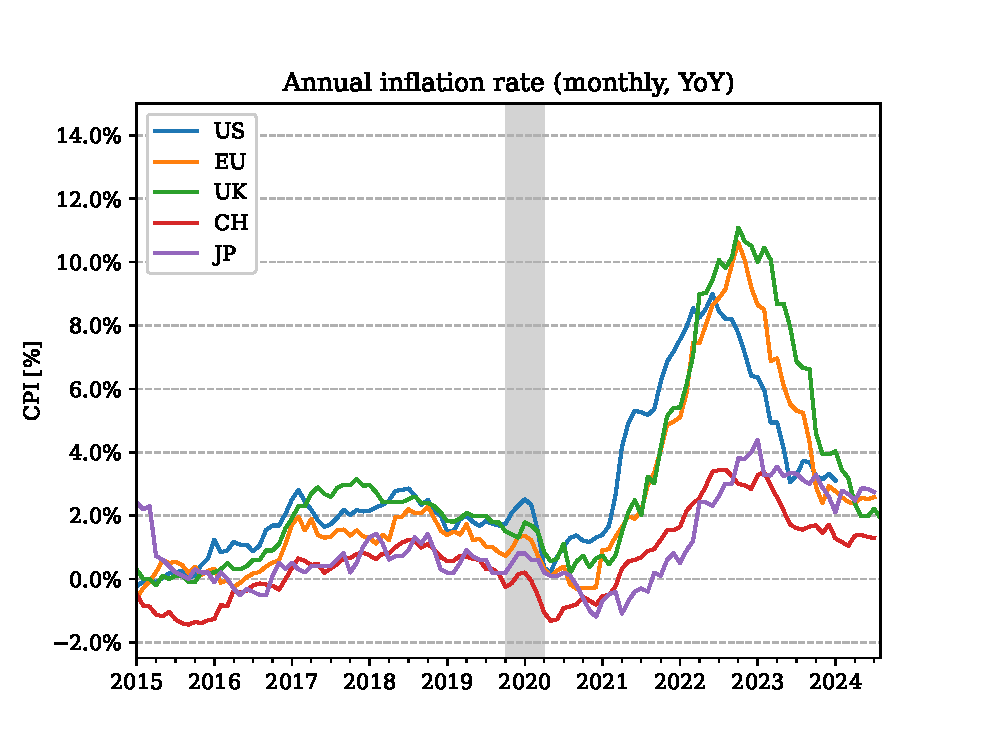
\includegraphics[width=\textwidth]{plots/inflation.eps}
        \caption{Tasa de inflación registrada (\textit{Consumer Price Index}).}
    \end{subfigure}
    \caption{Cambios en oferta monetaria e inflación para las diferentes áreas monetarias de interés durante el período 2015-2024. Fuente: elaboración propia.}
    \label{fig:m3-inflation}
\end{figure}


\subsubsection{Análisis de la velocidad de circulación del dinero}

En primer lugar se analiza la tendencia, variabilidad y estacionariedad de la velocidad de cirulación del dinero.

\begin{table}
    \centering
    \begin{tabular}{llllll}
        \toprule
        Magnitud                   & Estados Unidos & Eurozona & Suiza   & Reino Unido & Japón   \\
        \midrule
        $\mu_v$                    & -0.88\%        & -1.71\%  & -1.08\% & -1.60\%     & -1.79\% \\
        $\mu_v$ (hasta 2019.IV)    & -0.81\%        & -1.90\%  & -1.36\% & -1.48\%     & -2.02\% \\
        $\sigma_v$                 & 4.48           & 4.06     & 3.91    & 2.97        & 5.64    \\
        $\sigma_v$ (hasta 2019.IV) & 3.58           & 2.87     & 3.65    & 2.31        & 4.61    \\
        Valor-p                    & 0.002          & 0.000    & 0.001   & 0.000       & 0.000   \\
        \acrshort{adf} valor-p     & 0.031          & 0.038    & 0.012   & 0.017       & 0.062   \\
        \bottomrule
    \end{tabular}
    \caption{Parámetros obtenidos correspondientes a la velocidad de circulación del dinero para las diferentes áreas monetarias de interés}
    \label{tab:v-params}
\end{table}

Tal como muestra el Cuadro~\ref{tab:v-params}, la variación media ($\mu_v$) de la velocidad de circulación de dinero ($\Delta\log v_t$) es negativa para todas las áreas monetarias observadas y se mantiene en un intervalo relativamente uniforme entre el -1.79\% y el -0.81\% para la intervalo temporal analizado. La velocidad de dinero depende, en última instancia, de las preferencias de los agentes económicos en las diferentes áreas monetarias, y tal como se espera, se constatan diferentes pero uniformes cambios en la demanda de dinero a través de la variación en la velocidad de circulación. En todos los casos se descarta la hipótesis nula de que el valor medio de los cambios en la velocidad de cirulación sea nulo, con una confianza superior al 99\%.

Además, la variabilidad (expresada como desviación estándar $\sigma_v$), también es uniforme entre áreas monetarias, con un intervalo de entre 2.87 y 4.61.

Por último se analiza la estacionariedad de la serie temporal correspondiente a la variación del logaritmo de la velocidad de circulación. Para ello se hace uso del \acrfull{adf}, donde como se explicó en la sección correspondiente, la hipótesis nula es la existencia de una raíz unitaria en la serie temporal. Tal como muestra el Cuadro~\ref{tab:v-params}, se rechaza la hipótesis nula al 90\% y se concluye que no existe una raíz unitaria y que la serie es estacionaria.

Se plantea como trabajo futuro hacer uso del \acrfull{kpss} para confirmar la estacionariedad de la serie temporal.

\begin{figure}
    \centering
    \begin{subfigure}[b]{0.49\textwidth}
        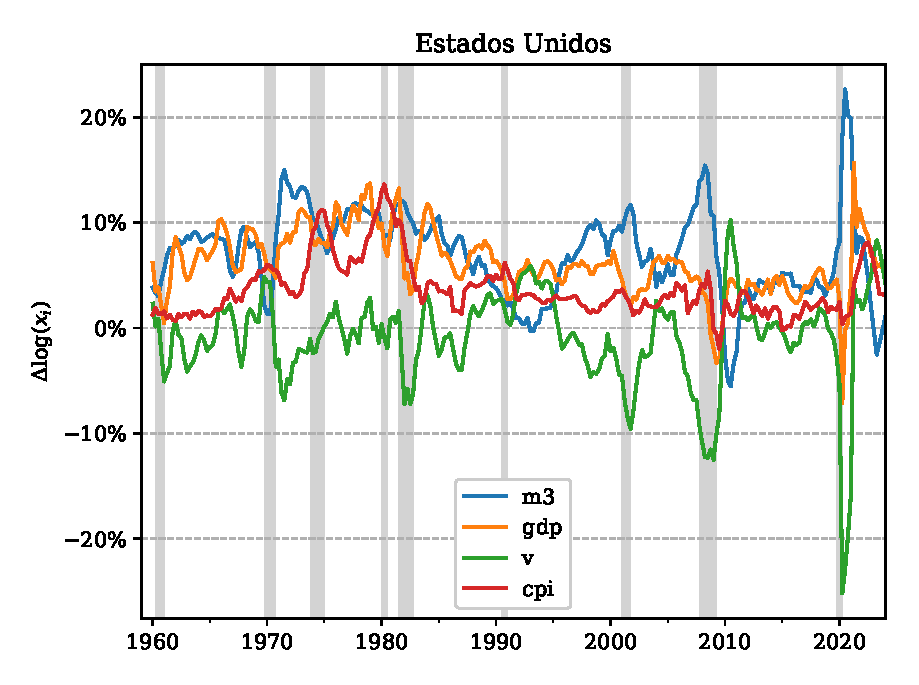
\includegraphics[width=\textwidth]{plots/us-magnitudes.eps}
        \caption{Estados Unidos}
    \end{subfigure}
    ~
    \begin{subfigure}[b]{0.49\textwidth}
        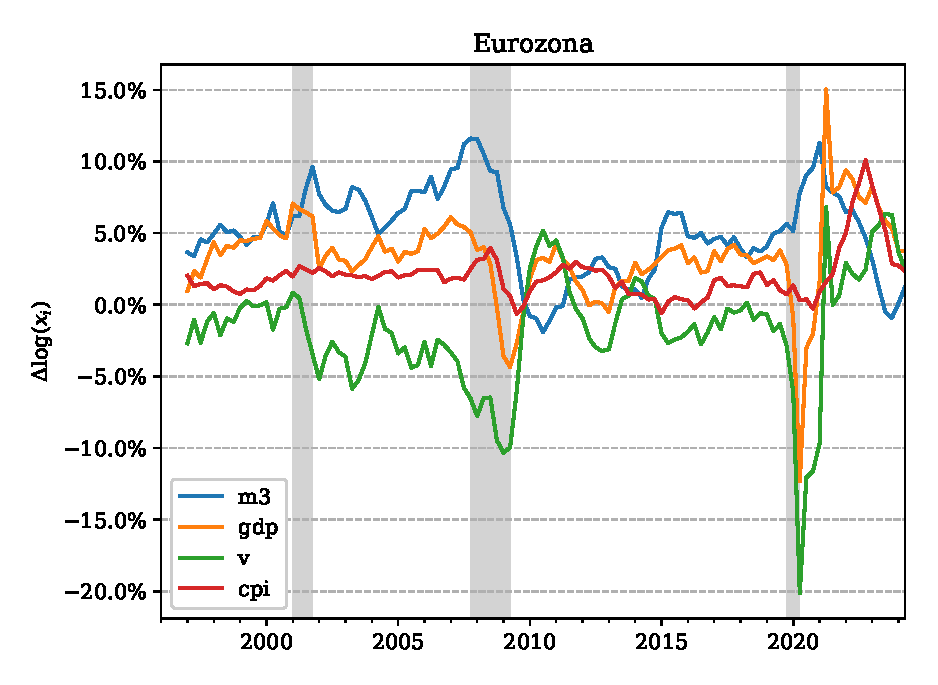
\includegraphics[width=\textwidth]{plots/eu-magnitudes.eps}
        \caption{Eurozona}
    \end{subfigure}
    ~
    \begin{subfigure}[b]{0.49\textwidth}
        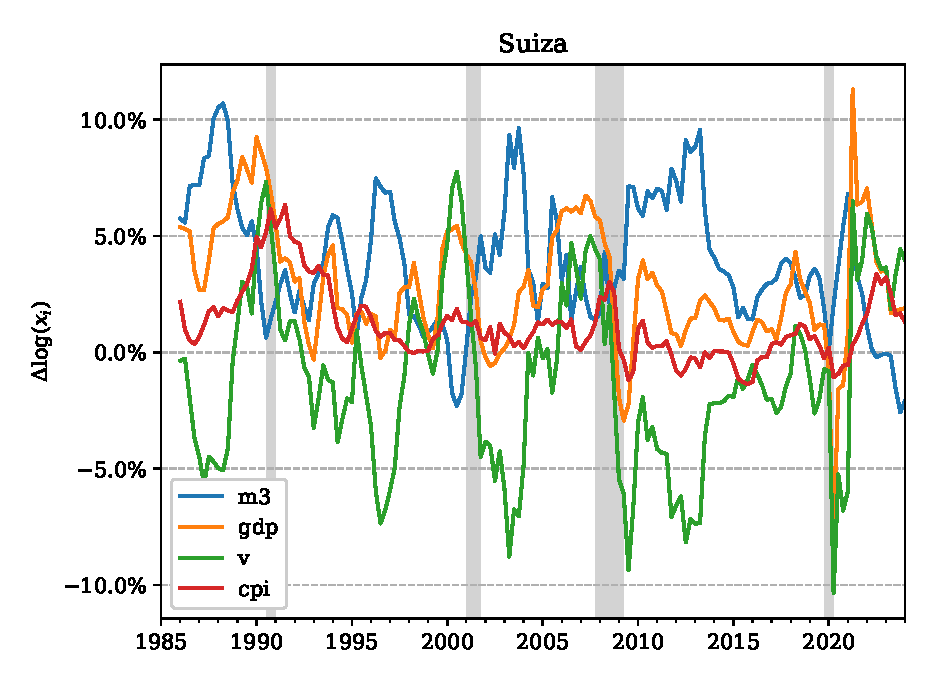
\includegraphics[width=\textwidth]{plots/ch-magnitudes.eps}
        \caption{Suiza}
    \end{subfigure}
    ~
    \begin{subfigure}[b]{0.49\textwidth}
        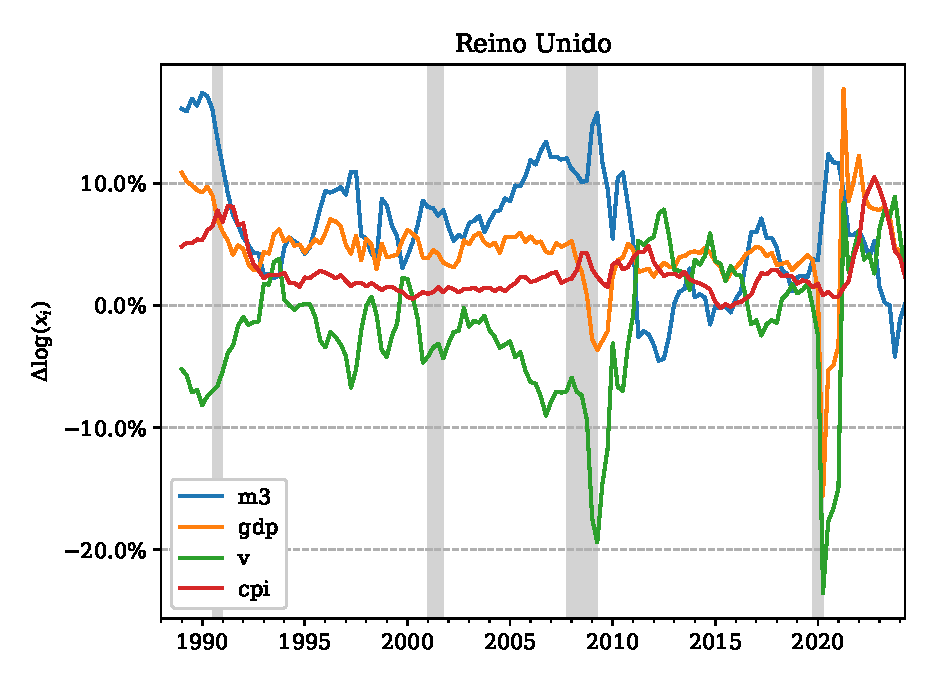
\includegraphics[width=\textwidth]{plots/uk-magnitudes.eps}
        \caption{Reino Unido}
    \end{subfigure}
    ~
    \begin{subfigure}[b]{0.49\textwidth}
        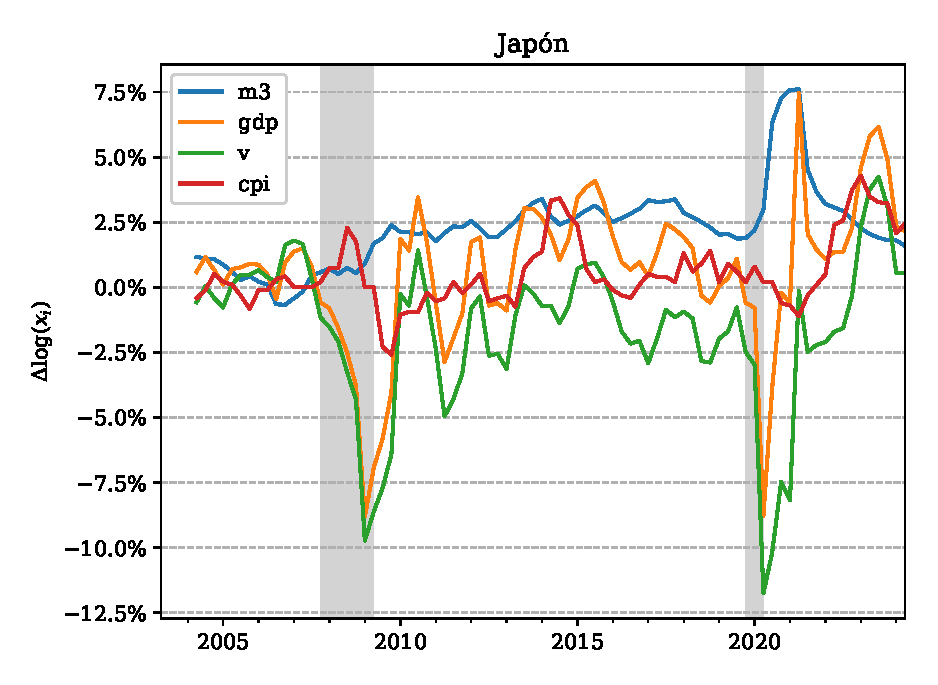
\includegraphics[width=\textwidth]{plots/jp-magnitudes.eps}
        \caption{Japón}
    \end{subfigure}
    \caption{Magnitudes registradas para las diferentes áreas monetarias de interés durante el período 2015-2024. Fuente: elaboración propia.}
    \label{fig:magnitudes}
\end{figure}

\subsubsection{Modelización de la velocidad de circulación del dinero}

De acuerdo con la teoría expuesta en la sección correspondiente, se modelan los cambios en la velocidad de circulación del dinero con un modelo de regresión markov con cambio de régimen. Tal como se especificó anteriormente, el modelo correspondiente a la variación del logaritmo de la velocidad de circulación del dinero se corresponde con la Ecuación~\ref{eq:markov-v}.


\begin{table}
    \centering
    \singlespacing
    \begin{tabular}{llllll}
        \toprule
        Magnitud                     & Estados Unidos & Eurozona & Suiza   & Reino Unido & Japón \\
        \midrule
        $\alpha_{S_1}$               & 0.002          & 0.035    & 0.030   & 0.009       & -     \\
                                     & (0.513)        & (0.000)  & (0.000) & (0.028)     & -     \\
        $\alpha_{S_2}$               & -0.109         & -0.023   & -0.033  & -0.085      & -     \\
                                     & (0.000)        & (0.000)  & (0.000) & (0.000)     & -     \\
        $\beta_{\mathrm{recession}}$ & -0.015         & -0.057   & 0.000   & -0.069      & -     \\
                                     & (0.025)        & (0.000)  & (0.960) & (0.000)     & -     \\
        $p_{00}$                     & 0.988          & 0.890    & 0.932   & 0.961       & -     \\
                                     & (0.000)        & (0.000)  & (0.000) & (0.000)     & -     \\
        $p_{10}$                     & 0.164          & 0.037    & 0.041   & 0.140       & -     \\
                                     & (0.059)        & (0.092)  & (0.050) & (0.042)     & -     \\
        $R^2$                        & 0.515          & 0.610    & 0.668   & 0.666       & -     \\
        \bottomrule
    \end{tabular}
    \caption{Parámetros obtenidos correspondientes al modelo de regresión de Markov correspondientes a la velocidad de circulación del dinero para las diferentes áreas monetarias de interés.}
    \label{tab:v-markov-params}
\end{table}


Los parámetros obtenidos en los diferentes modelos pueden se consultados en el Cuadro~\ref{tab:v-markov-params}. Los coeficientes son los correspondientes a la Ecuación~\ref{eq:markov-v}. La visualización del ajuste puede ser consultada en la Figura~\ref{fig:markov-v}.

Dado que el Banco de Japón publica únicamente los datos correspondientes al agregado monetario M3 a partir de 2003, se disponen de considerablemente menos datos que para el resto de áreas monetarias. Es por ello que el modelo regresivo de Markov correspondiente a la velocidad de circulación no consigue converger, indicándose correspondientemente en el Cuadro~\ref{tab:v-markov-params}.

Los valores p correspondientes al coeficiente relativo a la recesión indican que este es significativo al 95\%, excepto para el caso de Suiza (donde el modelo ajusta de diferente modo). Asimismo, todas las probabilidades de cambio de régimen son significativas al 90\%.

El coeficiente de determinación $R^2$ es una medida estadística que determina qué proporción de la variación de la variable dependiente puede ser explicada por las variables dependientes. En este caso se encuentran valores relativamente pobres (entre 0.515 y 0.668), pero que sí explican una parte significativa de la variación en los cambios de la velocidad de circulación del dinero.

\begin{figure}
    \centering
    \begin{subfigure}[b]{0.49\textwidth}
        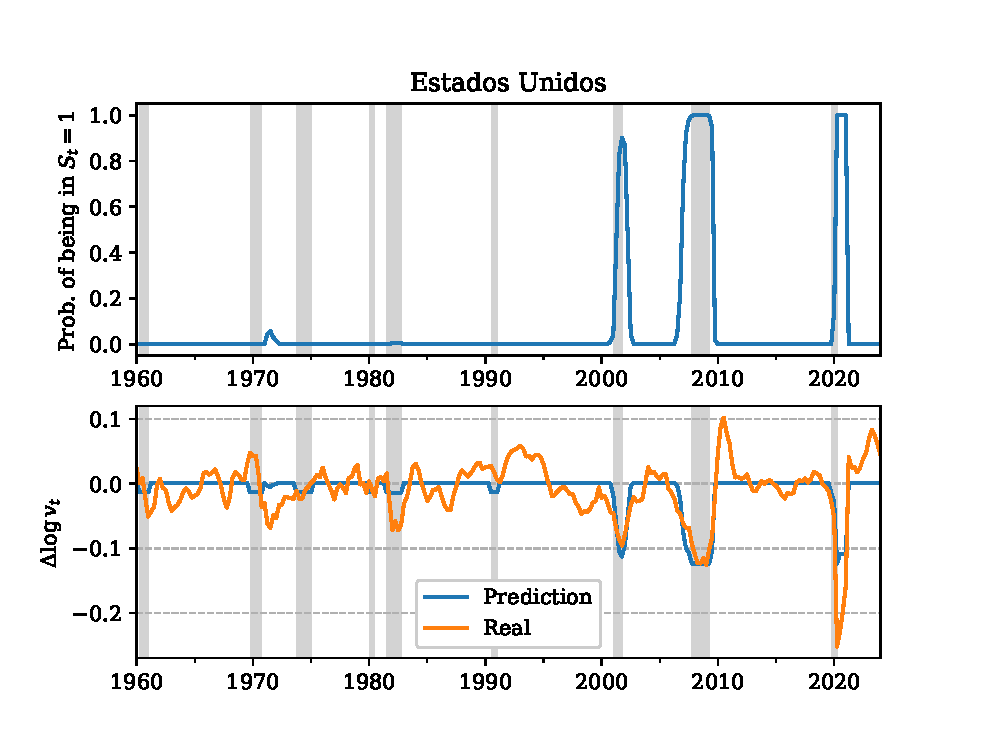
\includegraphics[width=\textwidth]{plots/us-markov-v.eps}
        \caption{Estados Unidos}
    \end{subfigure}
    ~
    \begin{subfigure}[b]{0.49\textwidth}
        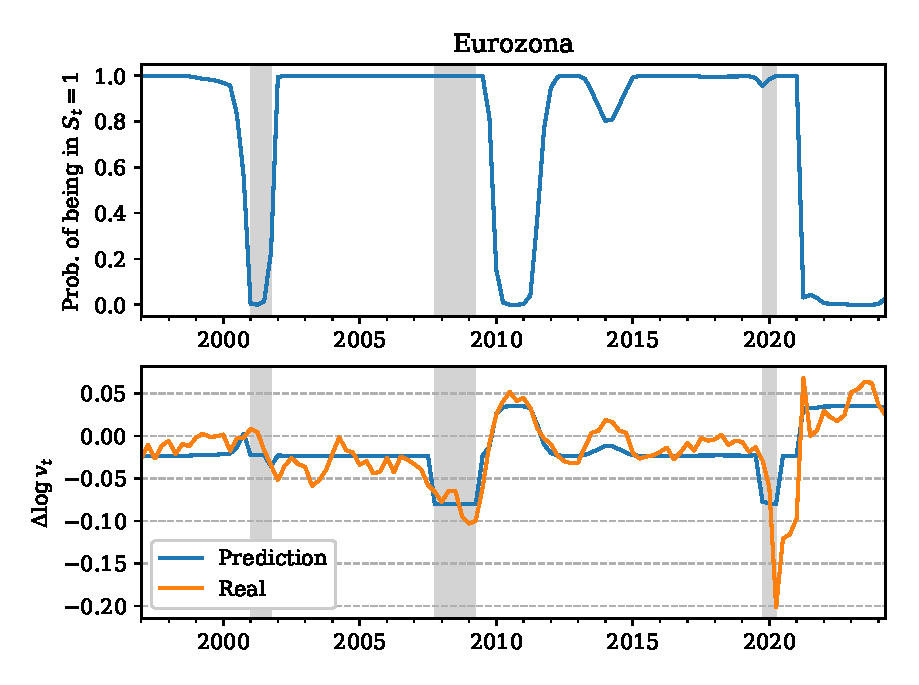
\includegraphics[width=\textwidth]{plots/eu-markov-v.eps}
        \caption{Eurozona}
    \end{subfigure}
    ~
    \begin{subfigure}[b]{0.49\textwidth}
        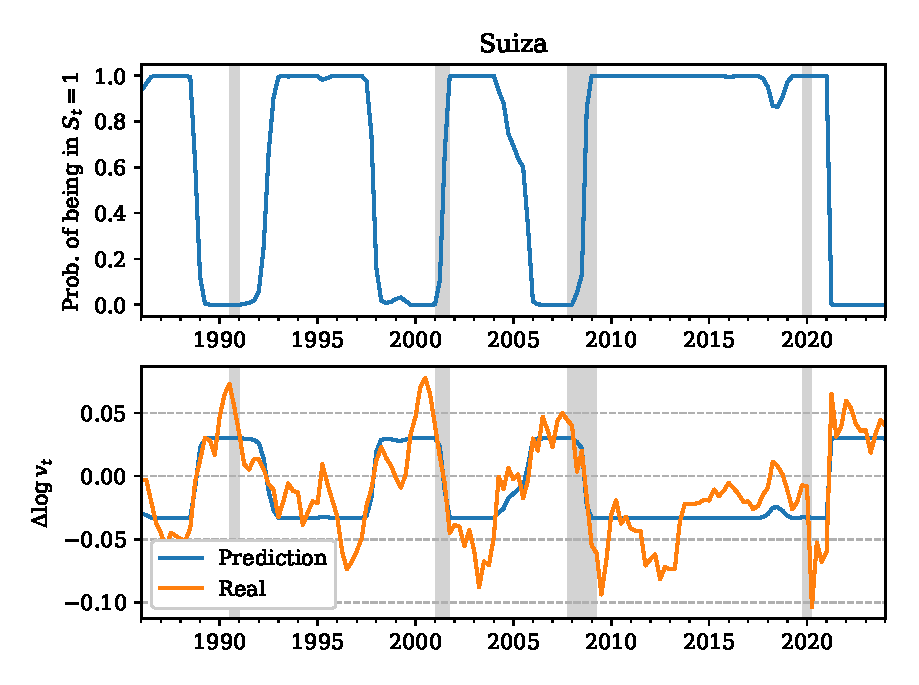
\includegraphics[width=\textwidth]{plots/ch-markov-v.eps}
        \caption{Suiza}
    \end{subfigure}
    ~
    \begin{subfigure}[b]{0.49\textwidth}
        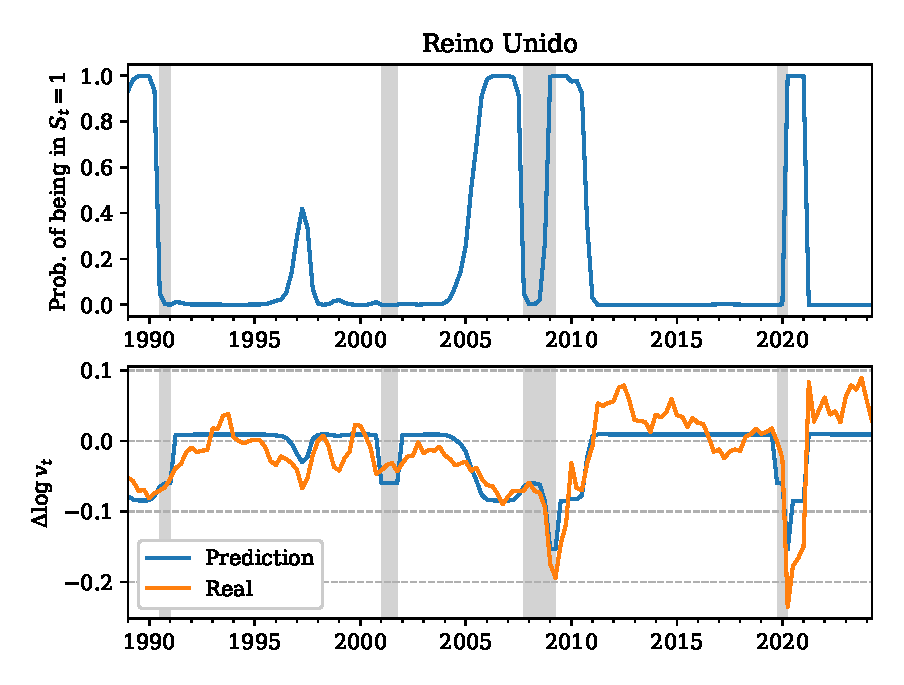
\includegraphics[width=\textwidth]{plots/uk-markov-v.eps}
        \caption{Reino Unido}
    \end{subfigure}
    ~
    \begin{subfigure}[b]{0.49\textwidth}
        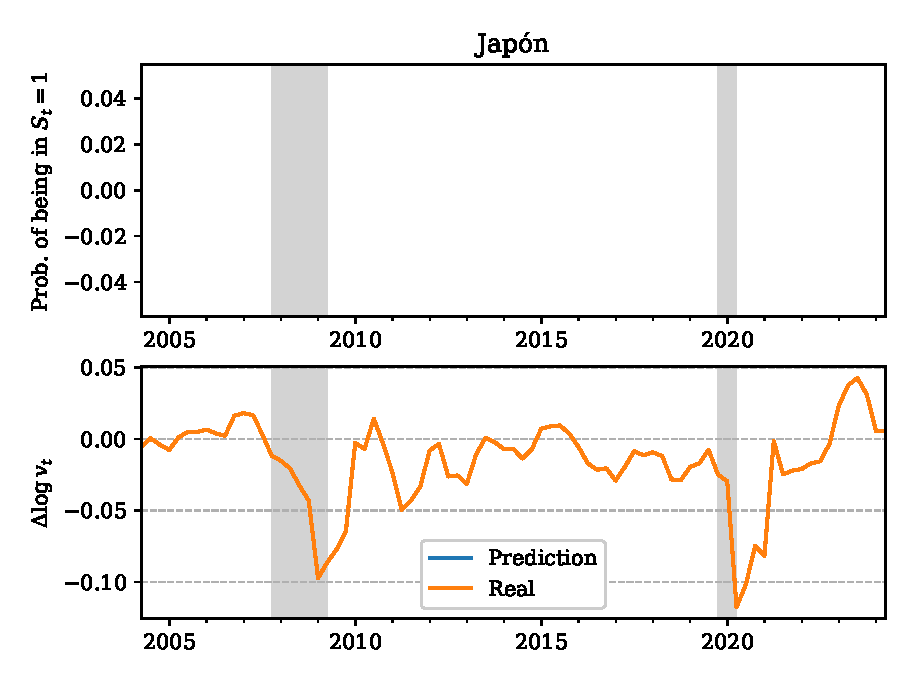
\includegraphics[width=\textwidth]{plots/jp-markov-v.eps}
        \caption{Japón}
    \end{subfigure}
    \caption{Probabilidad de encontrarse en el estado alto de Markov (arriba); valor real de la variación del logaritmo de la velocidad de circulación del dinero junto con la predicción del modelo (abajo).}
    \label{fig:markov-v}
\end{figure}

\subsubsection{Modelización de la inflación}

De acuerdo con la teoría expuesta en la sección correspondiente, se modela lla inflación con un modelo de regresión markov con cambio de régimen. Tal como se especificó anteriormente, el modelo correspondiente a la variación del logaritmo de la velocidad del nivel de precios $\Delta\log P_t$ se corresponde con la Ecuación~\ref{eq:markov-cpi}.


\begin{table}
    \centering
    \singlespacing
    \begin{tabular}{llllll}
        \toprule
        Magnitud          & Estados Unidos & Eurozona & Suiza   & Reino Unido & Japón   \\
        \midrule
        $c_{S_1}$         & 0.003          & 0.014    & 0.005   & 0.003       & 0.001   \\
                          & (0.153)        & (0.000)  & (0.001) & (0.223)     & (0.651) \\
        $\alpha_{0,S_1}$  & 0.191          & 0.130    & 0.071   & 0.098       & 0.162   \\
                          & (0.001)        & (0.000)  & (0.089) & (0.008)     & (0.001) \\
        $\alpha_{1, S_1}$ & 0.273          & 0.215    & 0.106   & 0.147       & 0.252   \\
                          & (0.074)        & (0.118)  & (0.245) & (0.143)     & (0.362) \\
        $\alpha_{2, S_1}$ & 0.154          & -0.003   & -0.023  & 0.120       & -0.129  \\
                          & (0.103)        & (0.977)  & (0.729) & (0.125)     & (0.375) \\
        $c_{S_2}$         & 0.053          & -0.017   & 0.044   & 0.018       & 0.017   \\
                          & (0.000)        & (0.001)  & (0.000) & (0.000)     & (0.022) \\
        $\alpha_{0,S_2}$  & -0.444         & 1.020    & 0.133   & 0.435       & 0.014   \\
                          & (0.004)        & (0.000)  & (0.058) & (0.000)     & (0.882) \\
        $\alpha_{1, S_2}$ & 0.217          & -0.502   & 0.053   & -0.069      & -0.992  \\
                          & (0.361)        & (0.034)  & (0.756) & (0.443)     & (0.501) \\
        $\alpha_{2, S_2}$ & 0.262          & 1.642    & -0.251  & 0.642       & 1.361   \\
                          & (0.244)        & (0.000)  & (0.085) & (0.000)     & (0.345) \\
        $\gamma_0$        & 0.100          & 0.034    & 0.076   & 0.051       & -0.002  \\
                          & (0.095)        & (0.376)  & (0.063) & (0.168)     & (0.958) \\
        $\gamma_1$        & -0.002         & -0.061   & 0.039   & 0.027       & 0.025   \\
                          & (0.982)        & (0.495)  & (0.566) & (0.702)     & (0.900) \\
        $\gamma_2$        & 0.096          & 0.054    & 0.083   & 0.035       & 0.028   \\
                          & (0.201)        & (0.213)  & (0.113) & (0.371)     & (0.665) \\
        $p_{00}$          & 0.977          & 0.957    & 0.993   & 0.972       & 0.955   \\
                          & (0.000)        & (0.000)  & (0.000) & (0.000)     & (0.000) \\
        $p_{10}$          & 0.116          & 0.218    & 0.043   & 0.060       & 0.150   \\
                          & (0.029)        & (0.040)  & (0.255) & (0.105)     & (0.107) \\
        $R^2$             & 0.819          & 0.836    & 0.789   & 0.811       & 0.817   \\
        \bottomrule
    \end{tabular}
    \caption{Parámetros obtenidos correspondientes al modelo de regresión de Markov correspondientes a la inflación para las diferentes áreas monetarias de interés.}
    \label{tab:cpi-markov-params}
\end{table}


Los parámetros obtenidos en los diferentes modelos pueden se consultados en el Cuadro~\ref{tab:cpi-markov-params}. Los coeficientes son los correspondientes a la Ecuación~\ref{eq:markov-cpi}. La visualización del ajuste puede ser consultada en la Figura~\ref{fig:markov-cpi}.

Es de interés resaltar que, de acuerdo con el Cuadro~\ref{tab:cpi-markov-params}, los valores de cambio en la oferta monetaria de períodos anteriores son significativos a la hora de modelizar la inflación presente (véanse los valores p correspondientes). Además, todas las probabilidades de cambio de régimen son significativas al 90\%, con la excepción del $p_{10}$ en Suiza, que merece un estudio independiente.

Los valores del coeficiente de determinación $R^2$ permiten concluir que el modelo es capaz de explicar con precisión la inflación a través de los cambios presentes y pasados de la oferta monetaria, presentando valores de entre $0.789$ y $0.836$.

\begin{figure}
    \centering
    \begin{subfigure}[b]{0.49\textwidth}
        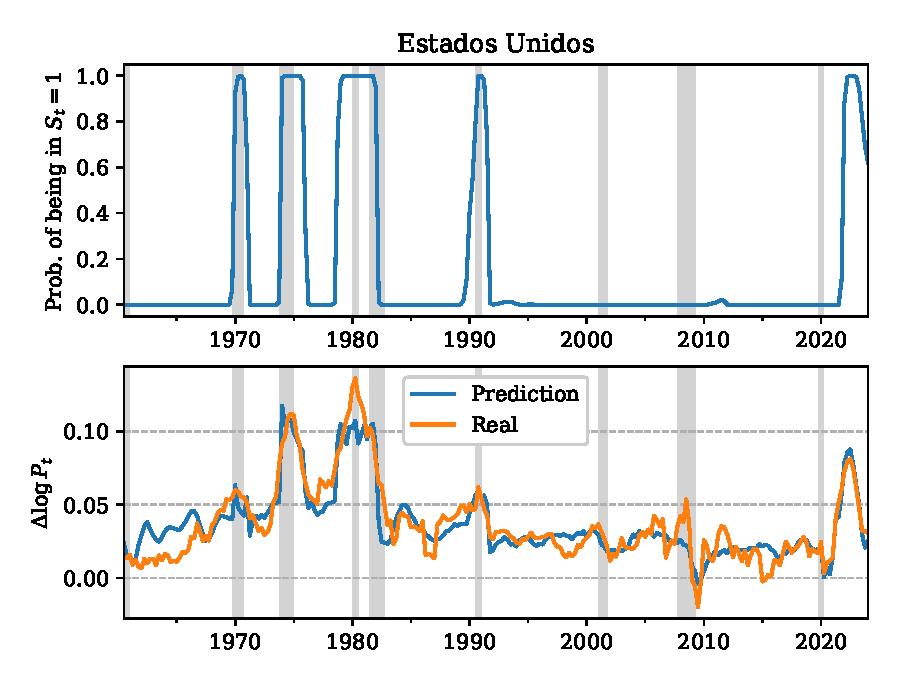
\includegraphics[width=\textwidth]{plots/us-markov-cpi.eps}
        \caption{Estados Unidos}
    \end{subfigure}
    ~
    \begin{subfigure}[b]{0.49\textwidth}
        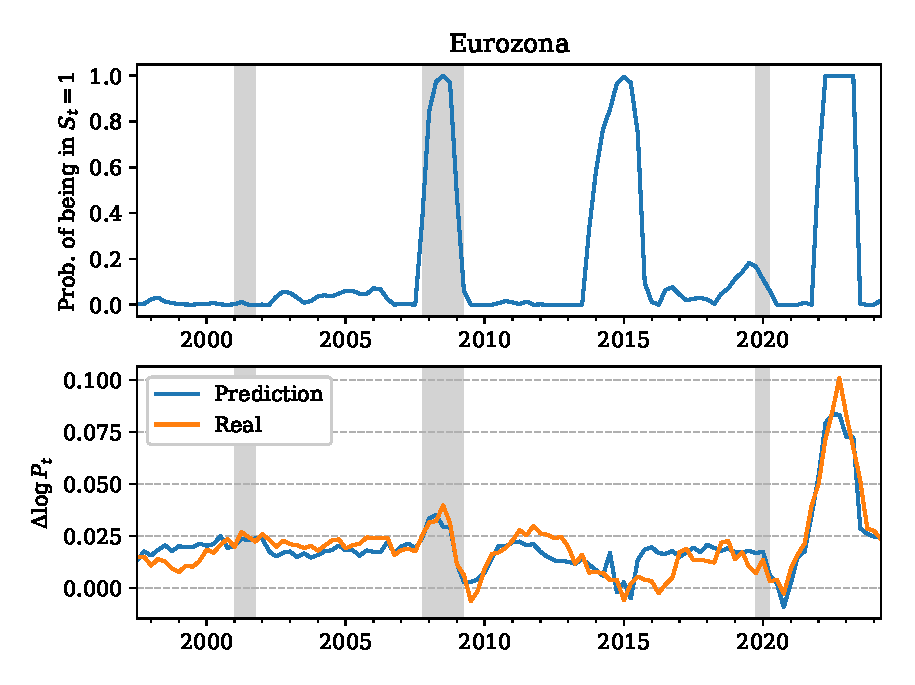
\includegraphics[width=\textwidth]{plots/eu-markov-cpi.eps}
        \caption{Eurozona}
    \end{subfigure}
    ~
    \begin{subfigure}[b]{0.49\textwidth}
        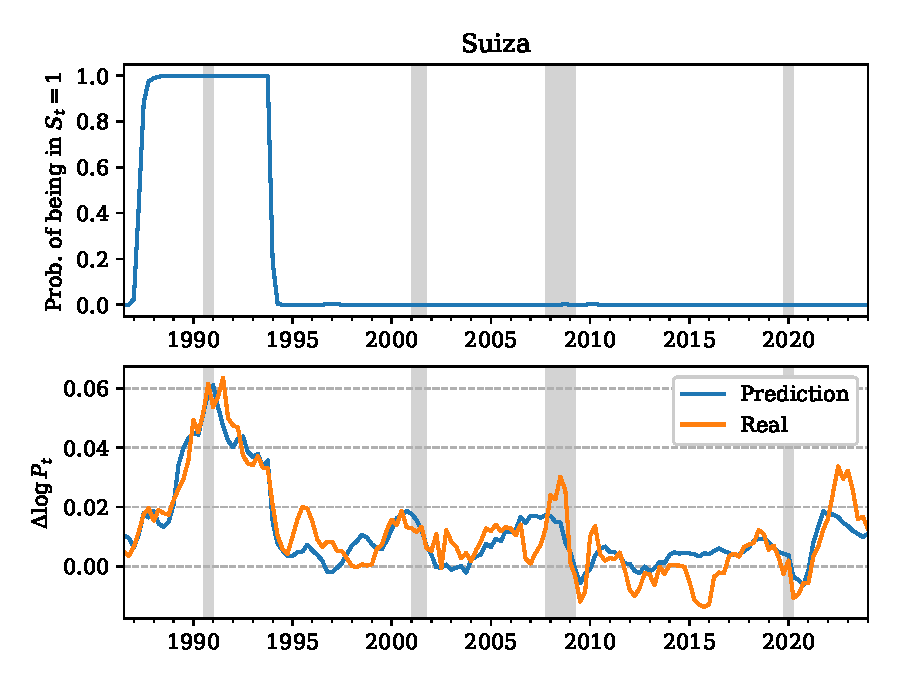
\includegraphics[width=\textwidth]{plots/ch-markov-cpi.eps}
        \caption{Suiza}
    \end{subfigure}
    ~
    \begin{subfigure}[b]{0.49\textwidth}
        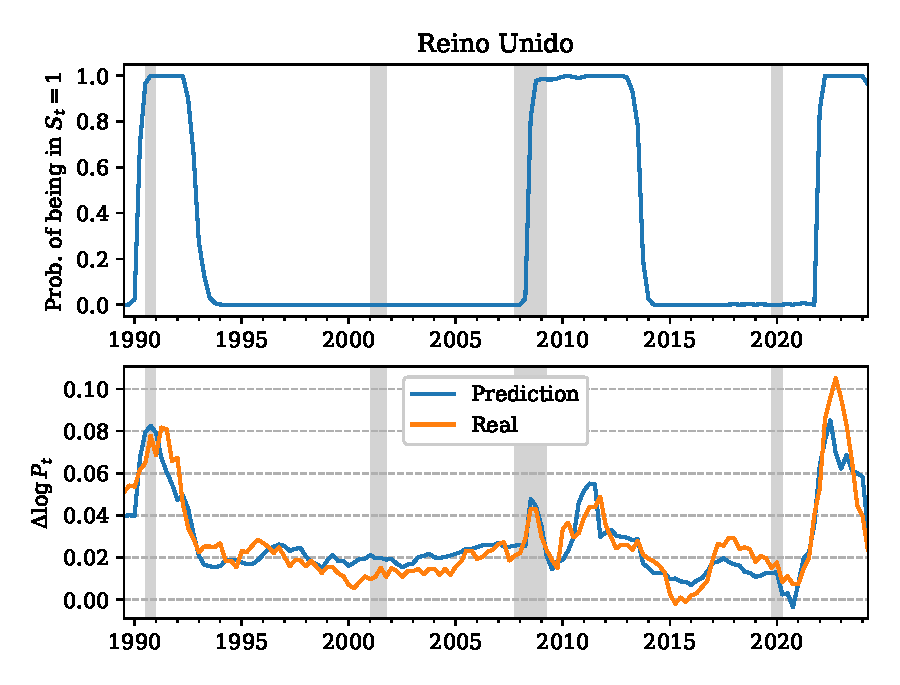
\includegraphics[width=\textwidth]{plots/uk-markov-cpi.eps}
        \caption{Reino Unido}
    \end{subfigure}
    ~
    \begin{subfigure}[b]{0.49\textwidth}
        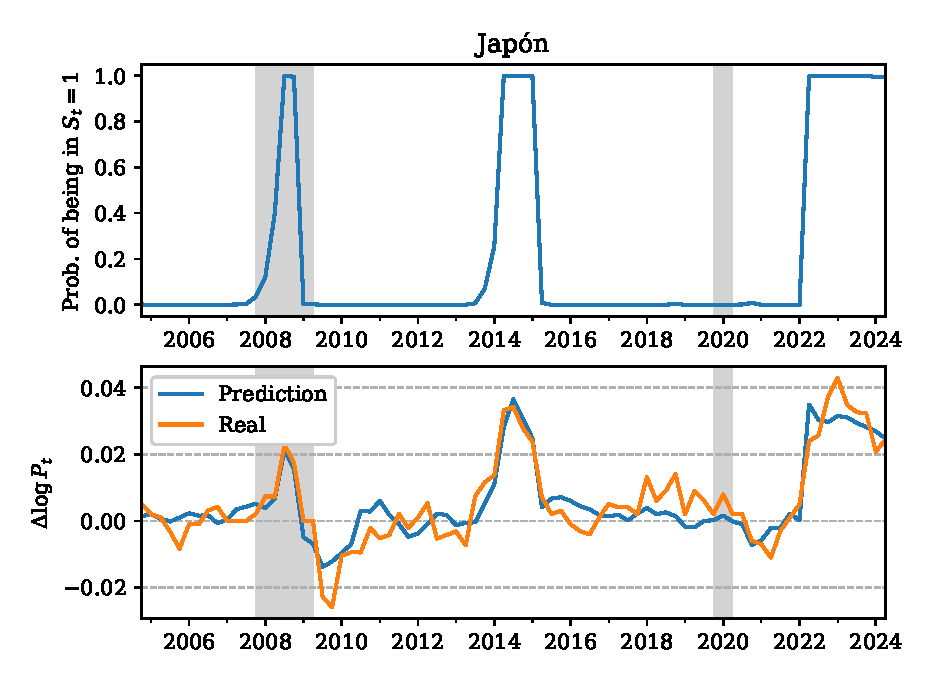
\includegraphics[width=\textwidth]{plots/jp-markov-cpi.eps}
        \caption{Japón}
    \end{subfigure}
    \caption{Probabilidad de encontrarse en el estado alto de Markov (arriba); valor real de la variación del logaritmo del nivel de precios junto con la predicción del modelo (abajo).}
    \label{fig:markov-cpi}
\end{figure}

\newpage
\subsection{Conclusiones}
El presente trabajo replica los resultados de la publicación correspondiente a \cite{castaneda2023}, donde se utilizan modelos similares de regresión de Markov. Este trabajo no sólo es capaz de replicar los resultados para el área monetaria de Estados Unidos, sino que también generaliza a modo de estudio controlado los resultados para otras áreas monetarias de interés: la Eurozona, el Reino Unido, Suiza y Japón.

Tras el análisis empírico se concluye que los cambios en la oferta monetaria correspondientes a los agregados monetarios en sentido amplio (M3 y M4x) explican una parte significativa de la variación en el nivel de precios (inflación). Además, se obtiene como resultado que no sólo son significativos los cambios en la oferta monetaria presente, sino también los cambios en la oferta monetaria pasada para determinar una correlación con la inflación.

Es de especial relevancia este último resultado para el diseño y la implementación de la política monetaria por parte de los bancos centrales. Buena parte de los principales bancos centrales en todo el mundo han usado la teoría correspondiente al modelo neokeynesiano (cf. Sección~\ref{modelo-neokeynesiano}), donde se resaltan como variables de interés la brecha de la producción (\textit{output gap}) y las expectativas de inflación como variables explicativas de la inflación. Sin embargo, tal como se ha analizado ampliamente en este trabajo, los cambios en la oferta monetaria en sentido amplio son significativos para explicar la inflación y no han de ser omitidos en el análisis.

Se concluye, por tanto, una recomendación a la banca central correspondiente a la incorporación de los agregados monetarios en sentido amplio como variables explicativas para la predicción y el análisis de la inflación, así como un más profundo análisis y revisión de los mecanismos de transmisión monetaria.

\nocite{*}
\newpage
\printbibliography

\newpage
\begin{appendices}
    \section{Fuentes de información}\label{fuentes-de-informacion}

En el presente trabajo se han usado múltiples fuentes de información, dependiendo del área monetaria y de la magnitud correspondiente.

A continuación se expone a modo de resumen una lista de las fuentes de datos consultadas y utilizadas por área monetaria:

Estados Unidos:
\begin{itemize}
  \item Gasto agregado: Reserva Federal. \textit{Gross Domestic Product, Quarterly, Billions of Dollars}. \url{https://fred.stlouisfed.org/series/GDP}.
  \item Oferta monetaria: M3 de ShadowStats. \url{http://www.shadowstats.com}.
  \item Inflación: Reserva Federal. \textit{Consumer Price Index for All Urban Consumers: All Items in U.S. City Average. Seasonally adjusted} (CPIAUCSL). \url{https://fred.stlouisfed.org/series/CPIAUCSL}.
\end{itemize}

Eurozona (datos del BCE):
\begin{itemize}
  \item Gasto agregado: dos opciones:
        \begin{itemize}
          \item \textit{Gross domestic product at market prices, Euro area 20 (fixed composition) as of 1 January 2023, Quarterly}. \url{https://data.ecb.europa.eu/data/datasets/MNA/MNA.Q.Y.I9.W2.S1.S1.B.B1GQ._Z._Z._Z.EUR.LR.N}.
          \item Utilizado: \textit{Gross domestic product at market prices, Euro area (Member States and Institutions of the Euro Area) changing composition, Quarterly}. \url{https://data.ecb.europa.eu/data/datasets/MNA/MNA.Q.N.U2.W2.S1.S1.B.B1GQ._Z._Z._Z.EUR.V.N}.
        \end{itemize}
  \item Oferta monetaria: \textit{Monetary aggregate M3 reported by MFIs, central gov. and post office giro institutions in the euro area (stocks), Euro area (changing composition), Monthly}. \url{https://data.ecb.europa.eu/data/datasets/BSI/BSI.M.U2.N.V.M30.X.1.U2.2300.Z01.E}.
  \item Inflación: HICP: \textit{HICP - Overall index, Euro area (changing composition), Monthly}. \url{https://data.ecb.europa.eu/data/datasets/ICP/ICP.M.U2.N.000000.4.INX}
\end{itemize}

Suiza (datos del SNB):
\begin{itemize}
  \item Gasto agregado: \texttt{gdpap\{BBIPS\}}.
  \item Oferta monetaria: M3 \texttt{snbmonagg\{GM3\}}.
  \item Inflación: diferentes opciones
        \begin{itemize}
          \item Utilizada: \textit{SNB National index (Dec. 2020=100)}. \texttt{plkopr\{LD2010100\}}.
          \item \textit{Eurostat HICP - monthly data (index)}. \url{https://ec.europa.eu/eurostat/databrowser/view/prc_hicp_midx/default/table?lang=en&category=prc.prc_hicp}
          \item \textit{IMF PCPIP: Inflation rate, averge consumer prices}. \url{https://data.imf.org/?sk=4ffb52b2-3653-409a-b471-d47b46d904b5}
        \end{itemize}
\end{itemize}

Reino Unido:
\begin{itemize}
  \item Gasto agregado: ONS \textit{Gross Domestic Product at market prices: Current price: Seasonally adjusted £m, quarterly}. \url{https://www.ons.gov.uk/economy/grossdomesticproductgdp/timeseries/ybha/pn2}.
  \item Oferta monetaria: BoE M4x, \textit{LPMAUYN, Monthly amounts outstanding of M4 (monetary financial institutions' sterling M4 liabilities to private sector) (in sterling millions) seasonally adjusted}. \url{https://www.bankofengland.co.uk/boeapps/database/FromShowColumns.asp?Travel=NIxAZxI1x&FromCategoryList=Yes&NewMeaningId=LM4,LM4L&CategId=6&HighlightCatValueDisplay=M4}.
  \item Inflación: ONS \textit{CPI INDEX 00: ALL ITEMS 2015=100}. \url{https://www.ons.gov.uk/economy/inflationandpriceindices/timeseries/d7bt/mm23}.
\end{itemize}

Japón:
\begin{itemize}
  \item Gasto agregado: Reserva Federal \textit{Gross Domestic Product for Japan. Billions of Yen,
          Seasonally Adjusted. Quarterly}. \url{https://fred.stlouisfed.org/series/JPNNGDP}.
  \item Oferta monetaria: BoJ \textit{M3/Average Amounts Outstanding/Money Stock} (\texttt{MD02'MAM1NAM3M3MO}). \url{https://www.stat-search.boj.or.jp/ssi/mtshtml/md02_m_1_en.html}.
  \item Inflación: e-Stat \textit{2020-Base Consumer Price Index. Monthly Report. 2024Jul.}. \url{https://www.e-stat.go.jp/en/stat-search/files?page=1&layout=datalist&toukei=00200573&tstat=000001150147&cycle=1&year=20240&month=23070907&tclass1=000001150149&result_back=1&tclass2val=0}.

\end{itemize}
\end{appendices}

\newpage

El presente Trabajo Fin de Máster ha sido elaborado por:

\vspace{3cm}

\textbf{Miguel González Calvo}

Madrid, 14 de octubre de 2024.

\end{document}
